\documentclass{article}

\usepackage{listings}
\usepackage[utf8]{inputenc}
\usepackage[greek,english]{babel}
\usepackage{alphabeta}
% Set page size and margins
% Replace `letterpaper' with `a4paper' for UK/EU standard size
\usepackage[letterpaper,top=2cm,bottom=2cm,left=3cm,right=3cm,marginparwidth=1.75cm]{geometry}

% Useful packages
\usepackage{amsmath}
\usepackage{graphicx}
\usepackage[colorlinks=true, allcolors=blue]{hyperref}
\usepackage{float} % Add the float package for better figure control

\title{Εργασία #1: Πλήρωση Τριγώνων}
\author{Βογιατζής Χαρίσιος ΑΕΜ:9192}

\lstset{frame=tb,
  language=Python,
  aboveskip=3mm,
  belowskip=3mm,
  showstringspaces=false,
  columns=flexible,
  basicstyle={\small\ttfamily},
  numbers=none,
  numberstyle=\tiny\color{gray},
  keywordstyle=\color{blue},
  commentstyle=\color{dkgreen},
  stringstyle=\color{mauve},
  breaklines=true,
  breakatwhitespace=true,
  tabsize=3
}

\begin{document}
\maketitle

\begin{abstract}
Σκοπός της εργασίας είναι η υλοποίηση αλγορίθμων πλήρωσης τριγώνων με flat shading και texture mapping.\\
Συγκεκριμένα παρουσιάζονται οι: Flat shading και Texture shading καθώς και τα αποτελέσματα που παράγουν.
\end{abstract}

\section{Εισαγωγή}
Έστω ότι το υπό εξέταση τρίγωνο ορίζεται από τις κορυφές του $p_k = (x_k, y_k) \in \mathbb{Z^2} , k = 0...2$ και τις πλευρές του $e_k, k = 0..2$, τότε μία γραμμή σάρωσης y τέμνει μόνο τις πλευρές $p_k$ για τις οποίες $y_{min} \leq y \leq y_{max}$. Συνεπώς μπορούμε να περιορίσουμε το τρίγωνο ανάμεσα σε δύο γραμμές σάρωσης. Κάθε γραμμή σάρωσης τέμνει ακριβώς 2 πλευρές του τριγώνου με εξαίρεση τις 2 ειδικές περιπτώσεις που ακολουθούν: \\
1. Γραµµές σάρωσης που αγγίζουν κορυφές\\
2. Γραµµές σάρωσης που διέρχονται από οριζόντιες πλευρές\\

\section{Flat shading}

\subsection{Αλγόριθμος}
Η συνάρτηση f\_shading(img, vertices, vcolors) δέχεται ως ορίσματα έναν καμβά, τις κορυφές των τριγώνων και τα χρώματα που τους αντιστοιχούν και επιστρέφει το χρωματισμένο καμβά.\\
Για το χρωματισμό του τριγώνου υπολογίζουμε το μέσο όρο των χρωμάτων των κορυφών του χρησιμοποιώντας τη συνάρτηση vector\_mean.

\begin{lstlisting}
def vector_mean(v1, v2, v3):
    """
    Calculates the mean of three vectors.
    """
    return (v1 + v2 + v3) / 3
\end{lstlisting}

Στη συνέχεια υπολογίζουμε τα $y_{min}$ και $y_{max}$ για να περιορίσουμε την περιοχή σάρωσης:

\begin{lstlisting}
ymin = max(int(np.floor(min(v0[1], v1[1], v2[1]))), 0)
ymax = min(int(np.ceil(max(v0[1], v1[1], v2[1]))), M-1)
\end{lstlisting}

Για κάθε γραμμή σάρωσης, βρίσκουμε τα σημεία τομής με τις πλευρές του τριγώνου:

\begin{lstlisting}
for y in range(ymin, ymax+1):
    intersections = []
    for i in range(3):
        p1 = triangle[i]
        p2 = triangle[(i + 1) % 3]
        y1, y2 = p1[1], p2[1]

        if y1 == y2:
            continue  # Skip horizontal edges

        if (y >= y1 and y < y2) or (y >= y2 and y < y1):
            x = p1[0] + (y - y1) * (p2[0] - p1[0]) / (y2 - y1)
            intersections.append(x)
\end{lstlisting}

Αν βρούμε ακριβώς 2 σημεία τομής, τα ταξινομούμε και χρωματίζουμε τα σημεία μεταξύ τους:

\begin{lstlisting}
if len(intersections) == 2:
    intersections.sort()
    x_start = max(int(np.ceil(intersections[0])), 0)
    x_end = min(int(np.floor(intersections[1])), width - 1)

    updated_img[y, x_start:x_end + 1] = flat_color
\end{lstlisting}

\section{Texture shading}

\subsection{Αλγόριθμος}
Η συνάρτηση t\_shading(img, vertices, uv, textImg) δέχεται ως ορίσματα έναν καμβά, τις κορυφές των τριγώνων, τις συντεταγμένες UV και την εικόνα texture και επιστρέφει το χρωματισμένο καμβά.\\
Χρησιμοποιούμε τη βοηθητική συνάρτηση vector\_interp για να πραγματοποιήσουμε γραμμική παρεμβολή των συντεταγμένων UV:

\begin{lstlisting}
def vector_interp(p1, p2, V1, V2, coord, dim):
    """
    Linearly interpolates vector V at a point `p` on the line segment from p1 to p2.
    V can be n-dimensional.
    """
    # Select the dimension
    c1 = p1[dim - 1]
    c2 = p2[dim - 1]

    # Handle division by zero (coordinates equal)
    if c1 == c2:
        return np.array(V1)

    # Interpolation factor
    t = (coord - c1) / (c2 - c1)

    # Linear interpolation
    return np.array(V1) + t * (np.array(V2) - np.array(V1))
\end{lstlisting}

Ο αλγόριθμος χωρίζεται σε δύο φάσεις:

\subsubsection{Φάση 1: Εύρεση σημείων τομής και συντεταγμένων UV}
Για κάθε γραμμή σάρωσης, βρίσκουμε τα σημεία τομής με τις πλευρές του τριγώνου και τις αντίστοιχες συντεταγμένες UV:

\begin{lstlisting}
for p1, p2, uv1, uv2 in edges:
    if p1[1] == p2[1]:
        continue  # Skip horizontal edges
        
    if (y >= min(p1[1], p2[1])) and (y <= max(p1[1], p2[1])):
        # Calculate x intersection
        x = vector_interp(p1, p2, p1[0], p2[0], y, 2)
        # Calculate UV coordinates at intersection
        uv_interp = vector_interp(p1, p2, uv1, uv2, y, 2)
        intersections.append(x)
        uvs.append(uv_interp)
\end{lstlisting}

\subsubsection{Φάση 2: Παρεμβολή συντεταγμένων UV και δειγματοληψία texture}
Για κάθε σημείο στη γραμμή σάρωσης, παρεμβάλουμε τις συντεταγμένες UV και δειγματοληπτούμε το χρώμα από την εικόνα texture:

\begin{lstlisting}
for x in range(x_start, x_end+1):
    # Interpolate UV coordinates based on x position
    uv_interp = vector_interp((x_start, y), (x_end, y), uv_start, uv_end, x, 1)
    u, v = uv_interp
    
    # Convert to texture coordinates
    tx = int(np.floor(u * (L - 1)))
    ty = int(np.floor(v * (K - 1)))
    
    # Sample texture using nearest neighbor
    img[y, x] = textImg[ty, tx]
\end{lstlisting}

\section{Η συνάρτηση render\_img}
Η συνάρτηση render\_img είναι η κύρια συνάρτηση που χειρίζεται την απόδοση των τριγώνων. Δέχεται ως ορίσματα:
\begin{itemize}
  \item faces: πίνακας με τις κορυφές των τριγώνων
  \item vertices: πίνακας με τις συντεταγμένες των κορυφών
  \item vcolors: πίνακας με τα χρώματα των κορυφών
  \item uvs: πίνακας με τις συντεταγμένες UV των κορυφών
  \item depth: πίνακας με το βάθος κάθε κορυφής
  \item shading: μεταβλητή ελέγχου για επιλογή Flat ή Texture συνάρτησης χρωματισμού
  \item textImg: η εικόνα texture για το texture mapping
\end{itemize}

Η συνάρτηση ακολουθεί τα εξής βήματα:
\begin{enumerate}
  \item Αρχικοποιεί τον καμβά με λευκό χρώμα
  \item Ταξινομεί τα τρίγωνα με βάση το μέσο βάθος των κορυφών τους (από πίσω προς τα μπροστά)
  \item Για κάθε τρίγωνο, εφαρμόζει την κατάλληλη συνάρτηση χρωματισμού (flat ή texture)
  \item Κανονικοποιεί τις τιμές των χρωμάτων στο διάστημα [0, 1]
  \item Μετατρέπει την εικόνα σε uint8 για αποθήκευση
\end{enumerate}

\begin{lstlisting}
def render_img(faces, vertices, vcolors, uvs, depth, shading, textImg):
    """
    Main rendering function that handles both flat and texture shading.
    """
    # Declare canvas size
    M = 512
    N = 512
    img = np.ones((M, N, 3), dtype=np.float32)

    # Sort faces by average depth (farthest to closest)
    avg_depth = np.mean(depth[faces], axis=1)
    sorted_indices = np.argsort(avg_depth)[::-1]  # Render from back to front

    for idx in sorted_indices:
        face = faces[idx]

        triangle_vertices = vertices[face]
        triangle_colors = vcolors[face]
        triangle_uvs = uvs[face] if uvs is not None else None

        if shading == 'f':
            img = f_shading(img, triangle_vertices, triangle_colors)
        elif shading == 't':
            img = t_shading(img, triangle_vertices, triangle_uvs, textImg)
        else:
            raise ValueError("Invalid shading mode. Use 'f' for flat or 't' for texture.")

    # Clamp values to [0, 1] before scaling to avoid overflows
    img = np.clip(img, 0, 1)

    # Normalize the canvas and convert it to the appropriate format for saving with OpenCV
    img_normalized = (img * 255).astype(np.uint8)

    return img_normalized
\end{lstlisting}

\section{Αποτελέσματα}

\begin{figure}[H] % Force figure placement exactly here
\centering
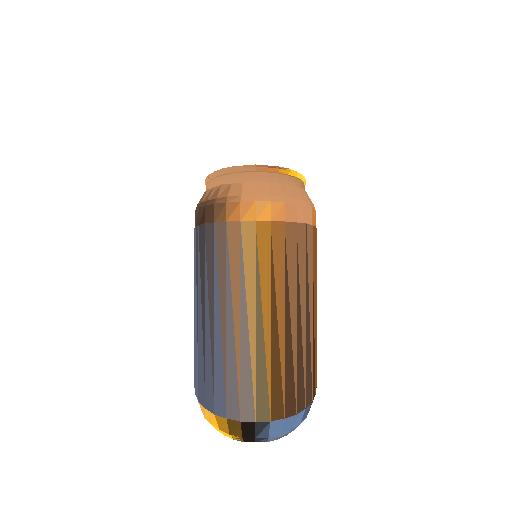
\includegraphics[width=0.3\textwidth]{flat_shading.png}
\caption{\label{fig:flat}Using Flat shading.}
\end{figure}

\begin{figure}[H] % Force figure placement exactly here
    \centering
    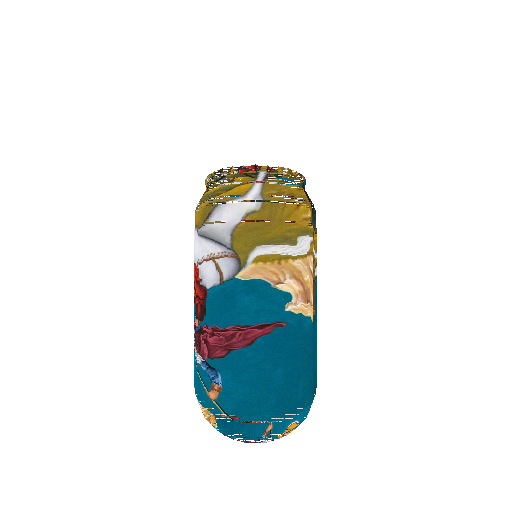
\includegraphics[width=0.3\textwidth]{texture_shading.png}
    \caption{\label{fig:texture}Using Texture shading.}
\end{figure}

\subsection{Προβλήματα Υλοποίησης}
Κατά τη διάρκεια της υλοποίησης αντιμετωπίσαμε ορισμένα προβλήματα:

\begin{itemize}
    \item \textbf{Προβλήματα Pixelation}: Παρατηρήσαμε προβλήματα pixelation στα όρια των τριγώνων, ιδιαίτερα στις γωνίες και στις ακμές. Αυτό οφείλεται στη χρήση της μεθόδου nearest neighbor για τη δειγματοληψία της texture, η οποία είναι απλή στην υλοποίηση αλλά δημιουργεί οπτικά artifacts.
    
\end{itemize}

\section{Κώδικας}
Μπορείτε να βρείτε τον κώδικα και τα αποτελέσματα στο \href{https://github.com/charisvt/cg-hw1-v4}{Github}.
\end{document}